\documentclass[a4paper,11pt]{article}
\usepackage{pos}
\usepackage{booktabs}  % For \toptrule etc.
\usepackage{xspace}
\usepackage[shortcuts]{extdash}  % For \Hyphdash* - Dash that disallows line break.
\newcommand{\eV}{\text{e\kern-0.15ex V}\xspace}
\newcommand{\GeV}{\text{G\eV}\xspace}
\graphicspath{{../img/code/}}

\title{A combined fit to the Higgs branching ratios at the International Large Detector at ILC}
\ShortTitle{Combined Higgs BRs at ILD}

\author*[a,\dag]{Jonas Kunath}

\affiliation[a]{Laboratoire Leprince-Ringuet, IN2P3-CNRS, École Polytechnique, Institut Polytechnique de Paris\\
Route de Saclay, 91120 Palaiseau, France}

\notes{
    \note{On behalf of the ILD concept group.}
}

\emailAdd{kunath@llr.in2p3.fr}

\abstract{
The Higgsstrahlung process as a Higgs boson production mechanism at a lepton collider
provides access to a high-purity Higgs boson sample.
The Higgs branching ratios can be measured simultaneously
by analysing the data inclusively.
For this purpose, we divide the sample into classes that
distinguish reasonably well between the Higgs decay modes.
These class counts are associated to the Higgs branching ratios through a
model-independent fit.
The fit provides an estimate for each of the Higgs branching ratios with
the full matrix of statistical correlations between the channels.
These are pure branching ratio measurements,
independent of any Higgs production mode cross section measurement.

We present a study on data simulated for the ILD concept
at the International Linear Collider (ILC) at 250~\GeV center-of-mass energy.
}

\FullConference{%
  *** Particles and Nuclei International Conference - PANIC2021 ***\\
  *** 5 - 10 September, 2021 ***\\
  *** Online ***
}

%% \tableofcontents

\begin{document}
\maketitle

\section{Introduction}
The International Linear Collider (ILC) will initially collide polarized beams
of electrons and positrons at center-of-mass energy $\sqrt{s}=250~\GeV$ (ILC250).
This energy will then be increased up to $\sqrt{s}=500~\GeV$~\cite{ILC_Staging_2017}.
The ILD concept group proposes the International Linear Detector~\cite{ILD_DBD,ILD_IDR}
as a detector for the ILC.
Its silicon trackers allow to measure impact parameters to less than 5~{\textmu}m~\cite{ILD_IDR}.
With the help of a Time Projection Chamber, transverse momenta of charged particles
can be measured with a resolution of $\sigma(1/p_T) = 2 \cdot 10^{-5}~\GeV^{-1}$~\cite{ILD_IDR}.
The highly granular electromagnetic and hadronic calorimeters
are based on the concept of Particle Flow
for track reconstruction and particle identification~\cite{ParticleFlow}.
A jet energy resolution of 3-4\% can be achieved~\cite{ILD_IDR}.
The surrounding coil provides a magnetic field of 3~T.

Here we focus on the Higgs boson production capabilities at the ILC250.
It will produce a large number of Higgs boson events.
The dominant Higgs production mode is Higgsstrahlung: $e^+e^- \to ZH$.
The background rates are low compared to hadron colliders.

One of the improvements compared to
a previously presented version of the study~\cite{LCWS_combined_Higgs}
is the inclusion of background processes in the result.

\section{Implementation}\label{sec:Implementation}
The samples used in this study were created by the ILD concept group since 2020.
More than 400.000 events were simulated for each of the nine main Standard Model (SM)
Higgs decay processes.
As background, we consider SM processes
with two or four fermions in the final state.
All events are weighted according to their SM cross sections
and to 2000~fb$^{-1}$ of integrated luminosity.
While this is the integrated luminosity from the 20-year running scenario,
the time would realistically be shared
between left-polarized
(80\% left-polarized electron beam, 30\% right-polarized positron beam)
and right-polarized (80\% right $e^-$, 30\% left $e^+$) runs.
Since this analysis is comparatively insensitive to beam polarization,
we simplify the analysis by considering only the left-polarized run.

The events are simulated for the ILC250 using the SetA beam parameters~\cite{ILC_Staging_2017}.
Leading order event generation is performed by WHIZARD 2.8.5~\cite{whizard,omega}.
Initial State Radiation, Beamstrahlung and Final State Radiation (FSR) are included.
The fragmentation and hadronization of final-state quarks and gluons
is performed with PYTHIA 6.422~\cite{pythia}.
The ILD detector geometry is described with DD4hep~\cite{DD4hep}
and simulated in GEANT4~\cite{GEANT4}.
Event reconstruction is performed with ILCSoft v02\Hyphdash*02, %~\cite{ILCSoft},
which includes PandoraPFA~\cite{PandoraPFA} for
the reconstruction of particle flow objects
and LCFIPlus~\cite{LCFIPlus} for flavor tagging.


\section{Event selection}\label{sec:selection}

We focus on Higgsstrahlung events in which the primary Z boson decays leptonically,
$Z \to e^+ e^-$ or $Z \to \mu^+ \mu^-$.
Event variables can be reconstructed after the isolated lepton pair is identified
and combined with FSR photon candidates.
Figure~\ref{fig:presel} shows the distribution of signal and background for
$Z \to \mu^+ \mu^-$ for the variables
that were built from the primary Z boson's decay products.
% The cuts from the previous steps are already applied in the subsequent steps.
Lepton colliders have the advantage that the initial state kinematics is known.
This is used when defining the recoil mass:
$M_{\mathrm{recoil}}^2 = s + M_Z^2 - 2\sqrt{s} \cdot E_Z$.
For signal events, the distribution peaks at $M_{\mathrm{recoil}} = M_{\mathrm{Higgs}}$.
The cuts presented in Figure~\ref{fig:presel} lead to a sample
with about 50\% purity at 50\% signal efficiency.
By definition, the efficiency is constant over Higgs decay modes
and the resulting sample is thus unbiased.

\begin{figure}[ht]
    \centering
    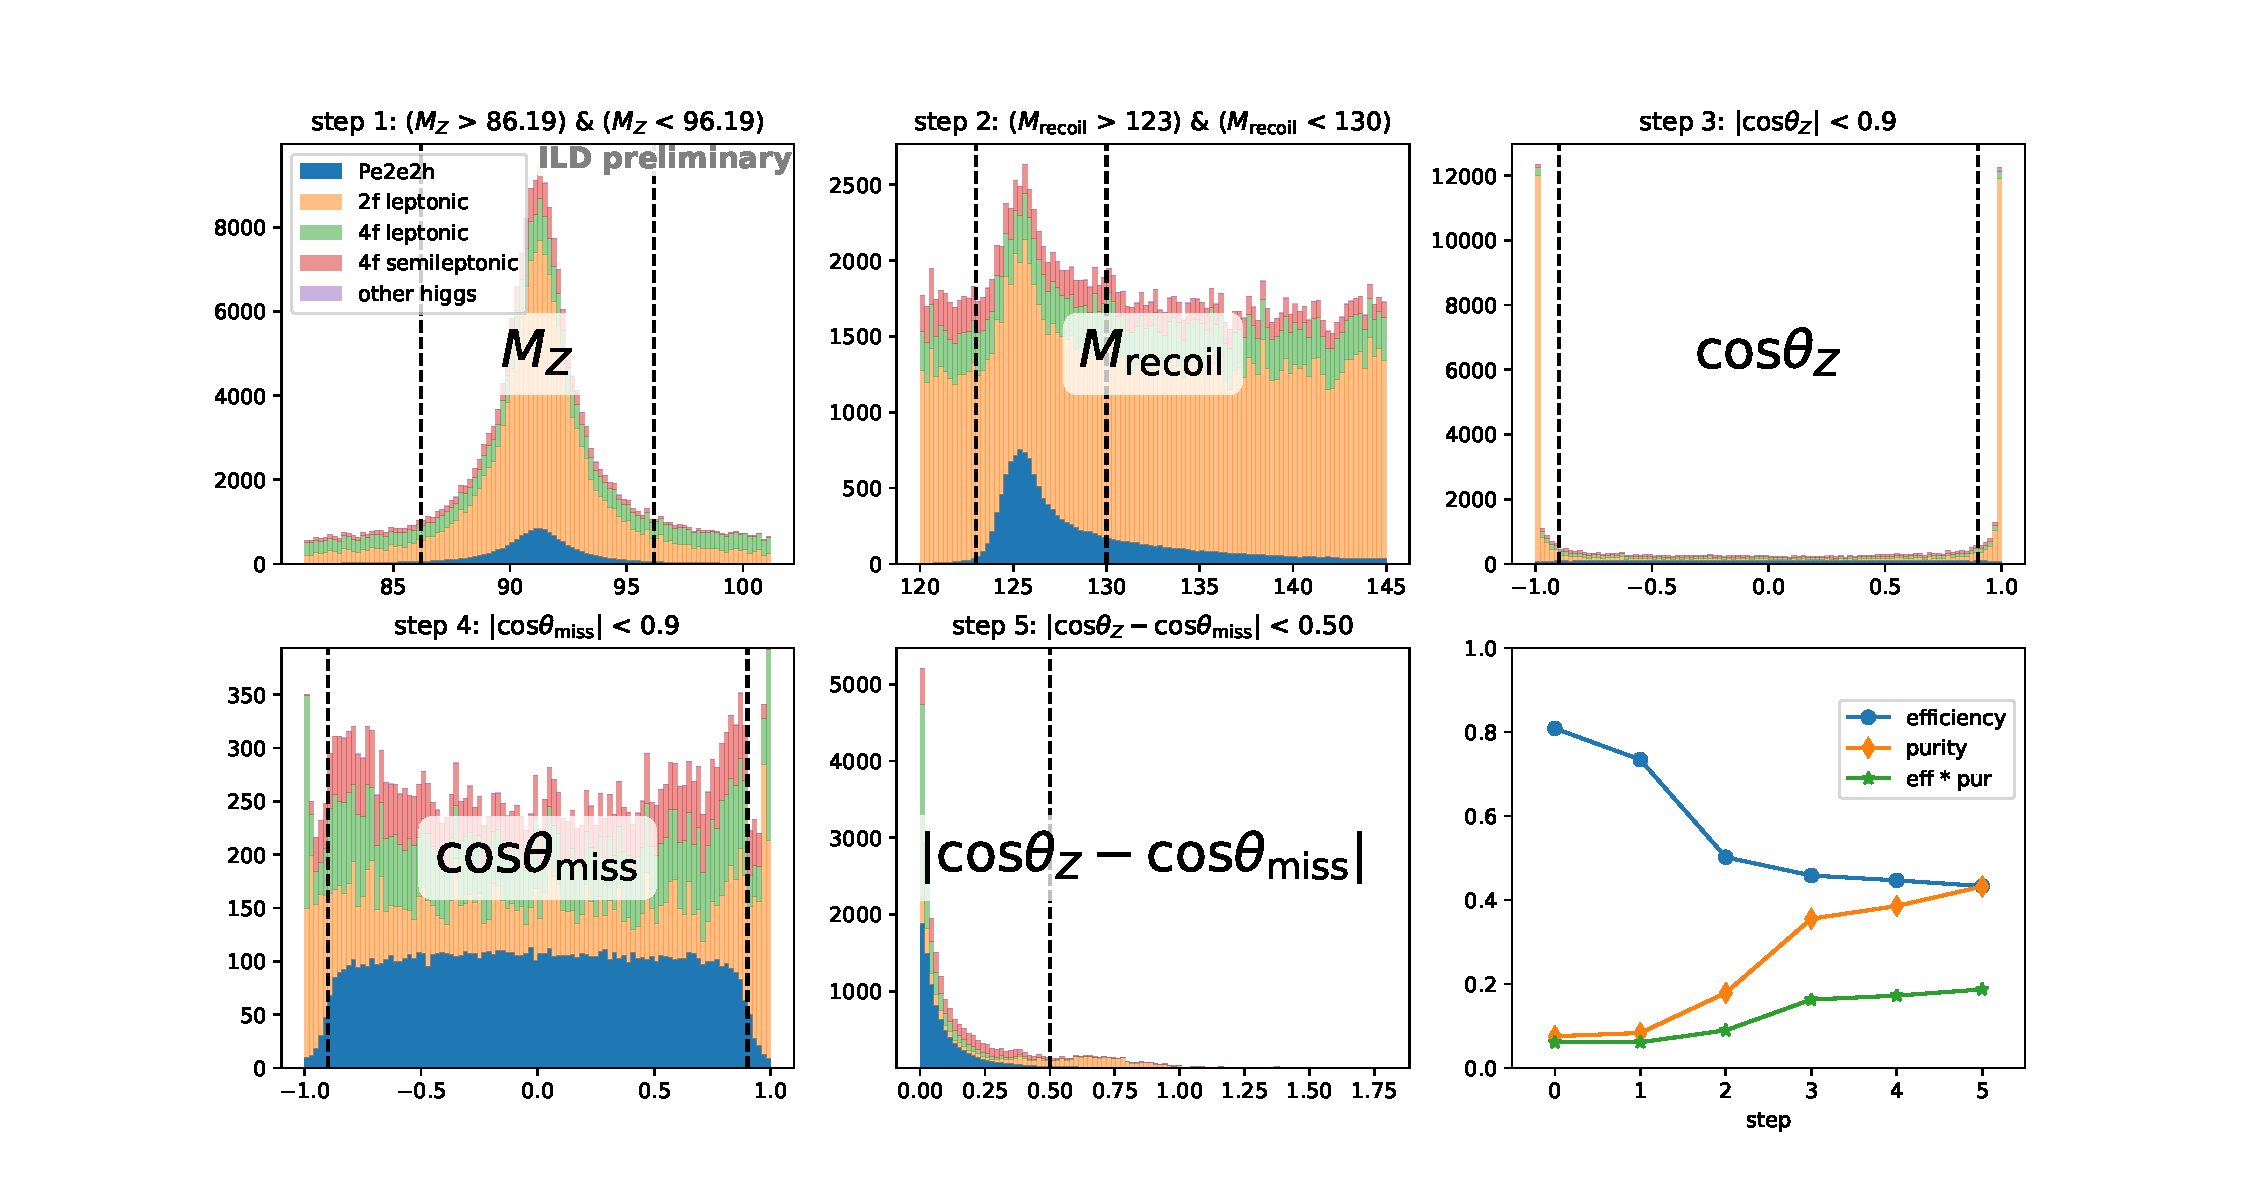
\includegraphics[width=0.9\textwidth, keepaspectratio]{presel_e2e2_for_proceedings}
    \caption{
        Cut flow for the event selection in the $Z \to \mu^+ \mu^-$ sample.
        The last figure shows the efficiency and purity after each step.
    }\label{fig:presel}
\end{figure}

We will now build a binned distribution of expected counts from the sample,
as shown in Figure~\ref{fig:box_counts}.
Each bin contains the events that fall into a specific class.
The class definitions can be found in the appendix of~\cite{LCWS_combined_Higgs}.
They were chosen so that they distinguish
relatively well between the considered Higgs decay modes.
The last bin contains all events that do not match any class definition.
The relative sensitivity to a Higgs decay mode varies between bins.
Next, we will present a fit that uses this variation in sensitivity
to derive the Higgs branching ratios.

\begin{figure}[ht]
    \centering
    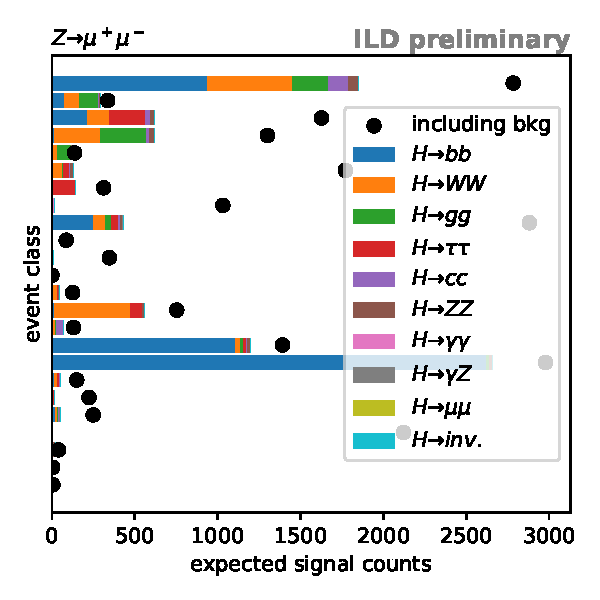
\includegraphics[width=0.43\textwidth, keepaspectratio]{intro_category_counts_w_bkg}
    \caption{
        Expected contributions per class from each of the Higgs decay modes
        assuming the Standard Model branching ratios.
        The black dots additionally contain the background contribution
        to the $Z \to \mu^+\mu^-$ Higgsstrahlung sample after event selection.
        The class definitions are described in the appendix of \cite{LCWS_combined_Higgs}.
    }\label{fig:box_counts}
\end{figure}

\section{Branching ratio uncertainties}\label{sec:fit}

\subsection{Setting up the fit}

\begin{figure}[ht]
    \centering
    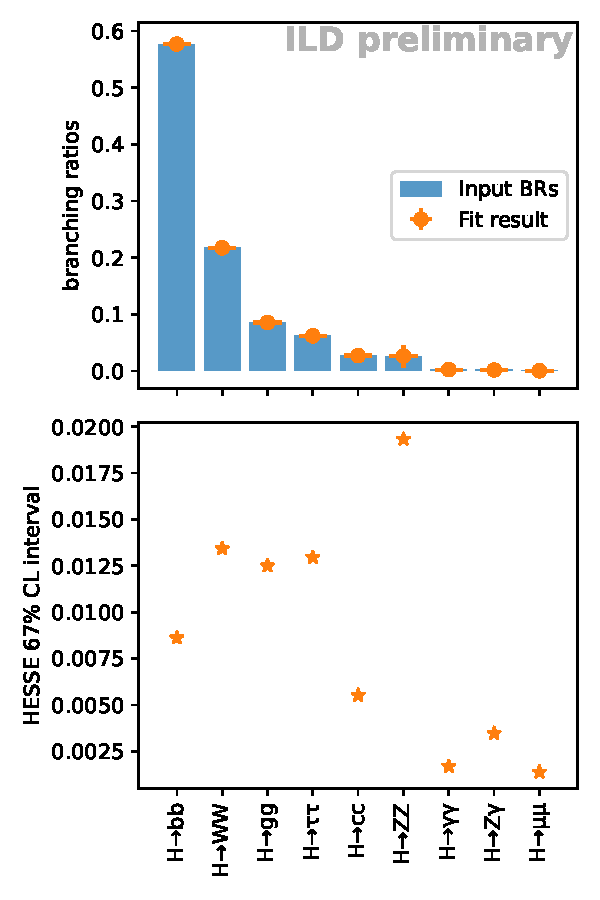
\includegraphics[width=0.38\textwidth, keepaspectratio]{br_estimates}
    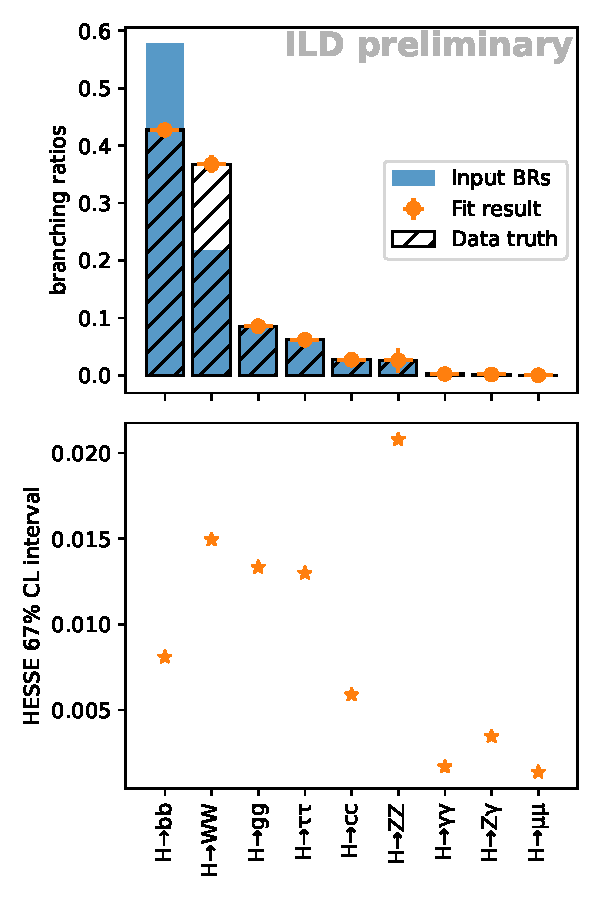
\includegraphics[width=0.38\textwidth, keepaspectratio]{changed_br_estimates}
    \caption{
        Top row: In blue, the BRs that were used in the simulation.
        The optimum of the fit and its uncertainty are indicated as orange error bars.
        The starting values of the fit are always the Standard Model Higgs BRs.
        The considered scenarios are the SM BRs (left)
        and a BSM scenario described in the text.
        For the BSM scenario, the BRs that were injected in the data sample
        are labeled as \textit{Data truth}.
        \\
        Bottom row: The absolute statistical uncertainties
        of the fit per branching ratio.
    }\label{fig:brs}
\end{figure}

The class probabilities for each Higgs decay mode or background process can
be determined using simulated events\footnote{
    The simulated events are needed both here and later on as a placeholder
    for the detector data.
    To prevent overfitting, we split the data set
    into two equal but statistically independent parts.
}
obtained by following the procedure outlined in Section~\ref{sec:Implementation}.
They are combined into a matrix, where each column corresponds to one process.
Applying the truth vector of the process counts to this matrix yields the class counts.
Conversely, given the class counts, a fit can be performed to gain access to the
process counts.
Only the relative contribution of each Higgs BR is taken as a free parameter.
% The fit is performed by \texttt{iminuit}~\cite{Minuit,iminuit}
% with a multinomial log-likelihood as its cost function.
With the nine BRs considered in the current analysis,
the fit provides the prediction for eight free parameters
and the corresponding $8 \times 8$ covariance matrix.
They can be converted into mean values and uncertainties for each of the BRs.

\subsection{Results}

\begin{figure}[ht]
    \begin{minipage}[c]{0.5\textwidth}
      \centering
      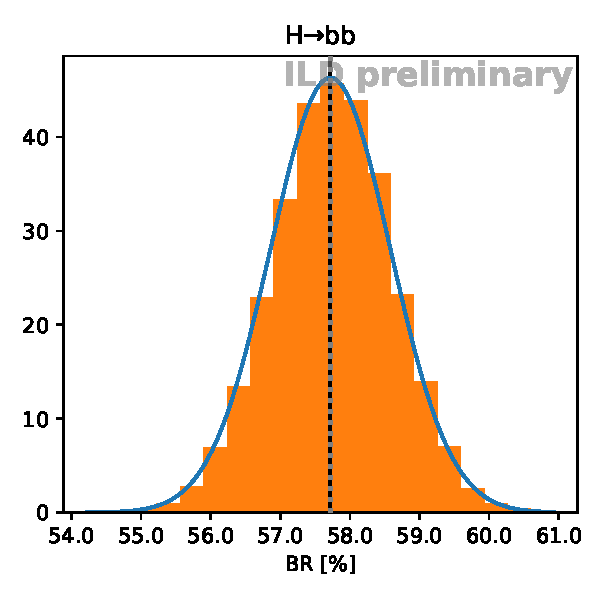
\includegraphics[width=0.9\textwidth, keepaspectratio]{toy_H_bb}
    \end{minipage}
    \begin{minipage}[c]{0.5\textwidth}
      \centering
      \begin{tabular}{lrr}
\toprule
{} &  SM BR &  $\sigma_{\mathrm{stat}}$ \\
\midrule
$H\to bb$           &  57.72 &                      0.86 \\
$H\to WW$           &  21.76 &                      1.34 \\
$H\to gg$           &   8.55 &                      1.25 \\
$H\to \tau\tau$     &   6.20 &                      1.30 \\
$H\to cc$           &   2.72 &                      0.55 \\
$H\to ZZ$           &   2.62 &                      1.93 \\
$H\to \gamma\gamma$ &   0.24 &                      0.17 \\
$H\to Z\gamma$      &   0.17 &                      0.35 \\
$H\to \mu\mu$       &   0.03 &                      0.14 \\
\bottomrule
\end{tabular}

    \end{minipage}
    \caption{
        Left: Validation of the uncertainty from
        a fit to the expected event counts scenario using a toy study.
        % \\
        Right:
        Preliminary results of a \texttt{MINUIT} fit to the expected event counts.
        The table gives the fitted values of the Higgs BRs
        and their absolute statistical uncertainties.
        All numbers are in percentages.
    }\label{fig:toys}
\end{figure}

Figure~\ref{fig:brs} gives the resulting values for a combination of the
$Z \to e^+e^-$ and $Z \to \mu^+\mu^-$ primary Z boson channels.
The left part of the figure shows the result in the SM case.
The right part of the figure supports the claim that the method
is truly model independent.
Here we assume a model with $BR(H \to b \bar{b})$ decreased by $15\%$,
and $BR(H \to W^+W^-)$ increased by $15\%$.
While this is an unrealistically large deviation from the SM, this shows that
the procedure still works far away from the SM hypothesis.

The results are validated in a toy study.
For this purpose we draw 10.000 class count vectors from a multinomial distribution
centered on the expected counts for each class.
The fit optimum for each toy is calculated and the corresponding BRs are stored
in histograms.
Figure~\ref{fig:toys} (left) displays the histogram for $H \to b \bar{b}$ in orange.
The blue Gaussian has as its mean value the optimum of the fit on the
expected event counts (EEC).
Its standard deviation is obtained through the covariance matrix of the fit
at the optimum.
The blue Gaussian and the histogram agree well, indicating that the EEC fit is stable.
The black line also indicates the position of the optimum of the EEC fit.
As expected, it agrees with the BR value that was
input to the simulation (dotted gray line).\footnote{
    Up to a small deviation due to the finite size of the simulated data sets.
}

The (absolute) $1 \sigma$-uncertainties are listed in the table on the right side
of Figure~\ref{fig:toys}.
These values assume BRs close to the SM expectation.
Additional non-SM Higgs decays
($H \to \textrm{invisible}$ $H \to \mu^+\tau^-, H \to b\bar{c}$, \ldots)
could be added to obtain explicit upper limits for them.


\section{Conclusion}\label{sec:conclusion}
The Higgsstrahlung process at a lepton collider allows the measurement of
all Higgs branching ratios (BRs) at once within the same unbiased sample.
At a Higgs factory such as the ILC250, the method presented in this contribution
can be applied to perform precision measurements of the observed BRs
and to obtain upper limits for additional Higgs decays.
It is a pure BR measurement, independent of any production cross section measurement.
The results can be combined with any analysis that does not use the
$ZH \to \left( e^+ e^-, \mu^+ \mu^- \right)$ channels.

%\appendix % switches the section numbering to letters instead of numbers
\acknowledgments
The authors would like to thank the LCC generator working group and the ILD software working
group for providing the simulation and reconstruction tools and producing the Monte Carlo
samples used in this study. This work has benefited from computing services provided by
the ILC Virtual Organization, supported by the national resource providers of the EGI
Federation and the Open Science GRID.

\bibliographystyle{JHEP}
\bibliography{refs.bib}

\end{document}
